\documentclass{article}

% NeurIPS 2024 style (preprint mode — no page limit, single-column title)
\usepackage[preprint]{neurips_2024}

\usepackage[utf8]{inputenc}
\usepackage[T1]{fontenc}
\usepackage{hyperref}
\usepackage{url}
\usepackage{booktabs}
\usepackage{amsfonts}
\usepackage{amsmath}
\usepackage{amssymb}
\usepackage{nicefrac}
\usepackage{microtype}
\usepackage{xcolor}
\usepackage{graphicx}
\usepackage{multirow}
\usepackage{makecell}    % for multi-line table headers
\usepackage{array}
\usepackage{bbm}         % for \mathbbm{1}
\usepackage{arydshln}    % for \hdashline in tables

% Convenience macros
\newcommand{\finrca}{\textsc{FINRCA}}
\newcommand{\frlg}{\textsc{FRLG}}
\newcommand{\aparca}{\textsc{APA-RCA}}
\newcommand{\synfrp}{\textsc{SynFRP}}
\newcommand{\indicator}{\mathbbm{1}}

\title{\finrca: Anomaly-Propagation-Aware Lineage Graph\\
       for Automated Root Cause Analysis\\
       in Financial Risk Pipelines}

\author{%
  Won Woo \\
  Department of Computer Science \\
  Hanyang University \\
  \texttt{thewoowon@hanyang.ac.kr}
}

\begin{document}

\maketitle

%----------------------------------------------------------------------
\begin{abstract}
Modern financial institutions are required under BCBS~239 to maintain
complete, accurate, and traceable data lineage across their risk reporting
pipelines.
Yet as of 2025, fewer than 10\% of globally systemically important banks
fully comply, with data lineage cited as the most persistent challenge.
When anomalies occur in multi-stage financial risk pipelines---spanning raw
market data ingestion, ETL transformations, feature engineering, and
regulatory reporting---identifying the root cause manually requires hours to
days of investigation.

We propose \finrca{}, a system that (1)~automatically constructs a
column-level \textbf{Financial Risk Lineage Graph~(FRLG)} from a risk pipeline
definition, and (2)~runs an \textbf{Anomaly-Propagation-Aware Root Cause
Analysis~(APA-RCA)} algorithm on the graph to identify root causes of observed
anomalies.
\aparca{} extends Random Walk with Restart~(RWR) with anomaly-score-weighted
transitions, transform-type-based edge weights, and ancestor-constrained
ranking.
A multi-signal anomaly detector---combining causal excess isolation, peer
deviation scoring, and short-long variance ratio analysis---provides the
anomaly scores that drive the walk.

We evaluate \finrca{} on the \synfrp{} benchmark: a synthetic financial risk
pipeline with controlled anomaly injection across seven anomaly types and three
pipeline scales (45--100+ nodes, 630 total runs).
\aparca{} v2 achieves \textbf{77.9\% overall Top-5} across all anomaly types---
outperforming Anomaly-Score Only (70.2\%) by 7.7~pp ($\chi^2=30.4$, $p<10^{-7}$)
and achieving 100\% on four of seven types.
A companion \emph{Schema-Constraint RCA} module resolves A4 aggregation errors
via FRLG structural integrity checks, achieving 100\% Top-1 with zero false
positives on other anomaly types.
The combined Hybrid achieves \textbf{91.9\% Top-5} and \textbf{59.5\% Top-1}
($\chi^2=111.7$, $p<10^{-25}$ vs.\ Anomaly-Score Only).
An expanded Real-Source Hybrid Benchmark (RSHB) covering 12 instruments
(10 US equities, 2 Korean Exchange equities, FX, and Treasury rates) over 756
trading days spanning three market regimes achieves 82.4\% Top-5
(+36.2~pp over Anomaly-Score Only), confirming robustness under
fat-tail conditions and cross-market heterogeneity.
Extended scalability confirms sub-20\,ms RCA query latency up to 1\,009-node pipelines.
\end{abstract}

%----------------------------------------------------------------------
\section{Introduction}
\label{sec:intro}

\subsection{The BCBS 239 Compliance Gap}

In 2013, the Basel Committee on Banking Supervision published BCBS~239
\cite{bis2013bcbs239}, mandating that banks ensure the accuracy,
completeness, and timeliness of their risk data, and demonstrate end-to-end
traceability from source systems to regulatory reports.

Over a decade later, the gap between regulation and practice remains striking.
BIS's 2025 implementation review \cite{bis2025review} reports that among 31
G-SIBs, \emph{only 2 institutions are in full compliance}, and no single
principle has achieved universal compliance.
The ECB's 2024 RDARR guide \cite{ecb2024rdarr} explicitly names
attribute-level data lineage as one of seven supervisory priority areas.
PwC's 2024 industry survey \cite{pwc2024bcbs} finds that structural data
governance deficiencies persist across the majority of G-SIBs.

The technical difficulty is real: financial risk pipelines are multi-stage,
with raw market data undergoing dozens of sequential transformations
---cleaning, currency conversion, feature engineering, risk metric
calculation---before reaching regulatory reports.
Each stage introduces potential failure points.
When a reported VaR figure is incorrect, finding which upstream transformation
introduced the error requires traversing a complex dependency graph, a task
that today remains largely manual.

\paragraph{FRTB 2025 raises the stakes further.}
The Fundamental Review of the Trading Book (FRTB), mandatory for G-SIBs from
January~2025 \cite{bis2019frtb}, substantially increases both the complexity
and the auditability requirements of risk pipelines.
Two FRTB provisions directly amplify the need for automated data lineage RCA.
First, the \emph{P\&L Attribution Test} (PLAT) requires firms to demonstrate
monthly that their Internal Model Approach (IMA) risk-theoretical P\&L closely
tracks the hypothetical P\&L computed from front-office pricing.
Failure causes automatic fallback to the Standardized Approach, which typically
carries 40--60\% higher capital requirements~\cite{bis2019frtb}.
A PLAT failure is, at its root, a data lineage discrepancy: some upstream
transformation produced figures inconsistent with the front-office source.
Identifying which node is the culprit is precisely the problem our system solves.
Second, FRTB's Sensitivity-Based Approach (SBA) mandates risk factor sensitivity
calculations (delta, vega, curvature) at the individual instrument level, adding
new computation layers to existing VaR pipelines---increasing node counts and
the manual RCA burden proportionally.
Our scalability experiments (Section~\ref{sec:experiments}) confirm that
\aparca{} remains below 20\,ms latency at 1\,009-node pipeline scales,
consistent with daily PLAT reporting windows.

\subsection{Motivation}

During employment at KB Kookmin Bank's StarBanking Operations Team, the author
directly observed the consequences of inadequate data lineage tooling.
When discrepancies arose in reported risk metrics, operational teams spent
hours to days tracing data flows across disparate systems, relying on tribal
knowledge and ad hoc SQL queries.
This experience motivates the central research question:

\begin{quote}
\emph{Can the root cause of a data quality anomaly in a financial risk
reporting pipeline be identified automatically, rapidly, and accurately
using a lineage graph?}
\end{quote}

\subsection{Contributions}

This paper makes six contributions:

\textbf{C1---FRLG.}
We define the \emph{Financial Risk Lineage Graph} schema for modeling
column-level data lineage in financial risk pipelines.
The schema captures five node types (Source, ETL, Feature, Risk, Report)
and four edge types (DirectMap, Filter, Calculate, Aggregate), reflecting
the structure of VaR/ES computation pipelines.
To our knowledge, this is the first column-level lineage graph schema
specifically designed for financial risk computation (as opposed to
general-purpose metadata catalogs such as OpenLineage or Apache Atlas).

\textbf{C2---Hop-Distance-Adaptive \aparca{}.}
We propose \emph{Anomaly-Propagation-Aware Root Cause Analysis} (v2), which
extends RWR with a novel hop-distance-adaptive weighting scheme: nodes close
to the observed anomaly target receive higher graph-structure trust, while
distant ancestors rely more on direct anomaly evidence.
This is the first RCA method to adapt RWR restart probability based on
hop distance in any domain; all prior graph-walk RCA methods (MicroRCA,
CloudRanger, CORAL, MULAN, REASON) use fixed transition weights.
A companion five-signal anomaly detector combines causal excess isolation,
peer deviation scoring, short-long variance ratio, rolling z-score, and
segment variance signals.

\textbf{C3---Schema-Constraint RCA.}
We introduce a lightweight ($O(|V|)$) structural integrity check on the FRLG
that detects aggregation schema violations (A4) with 100\% Top-1 accuracy and
zero false positives on non-A4 types---a complementary approach absent from
all existing RCA literature.

\textbf{C4---\synfrp{} Benchmark.}
We construct the \emph{Synthetic Financial Risk Pipeline} benchmark: a
configurable pipeline with GBM/Vasicek/RW-based data generation and a
controlled seven-type anomaly injection protocol with ground truth (630 runs).
To our knowledge, this is the first public benchmark for evaluating RCA
algorithms in the financial risk data lineage domain.

\textbf{C5---Anomaly Transfer Function (ATF) Framework.}
We derive a formal model of anomaly propagation through financial pipeline
transforms, yielding closed-form transfer coefficients $\rho_\tau$ per
transform type (Section~\ref{sec:atf}).
The ATF provides principled values for \aparca{}'s hop attenuation
($\alpha^* \approx 0.72$, matching the hand-tuned $\alpha = 0.7$) and
edge weights, explains why removing the hand-tuned $\beta$ improves
ablation performance, and derives a distribution-free temporal
discriminant $\phi_{\rm peer}$ that perfectly separates A3 code bugs
from A5 spike propagation on both synthetic and real data (0\% overlap).

\textbf{C6---Real-Source Hybrid Benchmark (RSHB).}
We validate on an expanded real-market dataset comprising 12 instruments
(US equities, Korean Exchange equities, FX, Treasury yields) over 756 trading
days spanning three market regimes (Fed tightening, banking stress, AI rally).
The RSHB is the first RCA evaluation benchmark built on actual financial market
data from two distinct equity markets.

%----------------------------------------------------------------------
\section{Related Work}
\label{sec:related}

\paragraph{Data lineage systems.}
Cheney et al.~\cite{cheney2009provenance} provide a foundational survey of
data provenance in databases, distinguishing why-, where-, and
how-provenance.
Davidson and Freire~\cite{davidson2008provenance} survey provenance in
scientific workflows.
Industrial tools---Apache Atlas, OpenLineage, Atlan, Solidatus---provide
lineage visualization and governance, but none offers RCA capability, and
none has been evaluated with published RCA accuracy metrics.
No academic work has addressed lineage-based RCA in the financial risk domain.

\paragraph{Root cause analysis.}
RCA has been extensively studied in cloud and microservices contexts.
MonitorRank~\cite{kim2013monitorrank} pioneered random walk on sensor dependency
graphs at LinkedIn, establishing the core propagation-walk paradigm.
CloudRanger~\cite{wang2018cloudranger} applied second-order random walk on PC-algorithm
causal graphs for cloud-native systems.
MicroRCA~\cite{wu2020microrca} introduced Personalized PageRank on attributed
service topology graphs (89\% precision), becoming the canonical graph-walk RCA reference.
GROOT~\cite{wang2021groot} deployed GrootRank (a PageRank variant) on event causal
graphs in production e-commerce at 78\% Top-1.
More recent methods include CIRCA~\cite{li2022circa} (causal Bayesian network with
intervention recognition at KDD 2022), CORAL~\cite{wang2023coral} and
REASON~\cite{wang2023reason} (both KDD 2023: incremental/hierarchical causal graph + RWR),
MULAN~\cite{zheng2024mulan} (multi-modal causal learning + RWR, WWW 2024),
Nezha~\cite{yu2023nezha} (multi-modal event graph, FSE 2023), and
Chain-of-Event~\cite{yao2024chainofevent} (weighted event causal graph from deployment
history, FSE 2024 industry).
RCACopilot~\cite{chen2024rcacopilot} uses LLMs for incident root-cause generation.
BARO~\cite{pham2024baro} applies Bayesian change-point detection.
AERCA~\cite{xiao2025aerca} (ICLR 2025 Oral) uses Granger causal discovery to
identify anomaly-introducing interventions in time series.
RCAEval~\cite{pham2025rcaeval} provides the most comprehensive benchmark.
Wang and Qi~\cite{wang2024rcasurvey} survey 100+ methods through 2024.

All of the above target \emph{system failures} (service crashes, latency spikes,
resource exhaustion) in microservice/cloud environments.
None addresses data quality anomalies propagating through financial risk
computation pipelines, and none uses data lineage graphs as the propagation
substrate.
Furthermore, while multiple methods use RWR or PageRank as the localization walk,
none adapts the restart probability as a function of hop distance from the observed
anomaly target---FINRCA's primary algorithmic contribution.

Li et al.~\cite{li2024gnn} (GNN-based root cause localization for general data
pipelines) and Assaad et al.~\cite{assaad2023rootcause} (acyclic causal graph
methods for time series anomalies) are the closest prior work in terms of problem
framing, but neither targets financial regulatory pipelines nor provides a
domain-specific anomaly taxonomy.
Wang et al.~\cite{wang2023hierarchical} propose hierarchical GNNs for causal
discovery.
Our work differs in domain specificity (financial risk pipelines, BCBS 239),
algorithm design (hop-distance-adaptive typed-edge RWR with multi-signal detector),
and the provision of a reproducible benchmark with seven financial anomaly types
and real-source validation across two equity markets (US + KRX).

\paragraph{Graph-based propagation.}
Tong et al.~\cite{tong2006rwr} establish the theoretical foundations of RWR
on graphs.
\aparca{} extends RWR with three domain-specific modifications described in
Section~\ref{sec:algorithm}.

\paragraph{OpenLineage to FRLG schema mapping.}
A key practical concern is whether FINRCA can ingest lineage metadata produced
by existing tools without manual re-engineering.
Table~\ref{tab:openlineage} shows the field-level mapping between the
OpenLineage \texttt{RunEvent} schema~\cite{openlineage} and the FRLG node/edge
schema.
Each OpenLineage \texttt{Job} (a transformation step) maps to a single FRLG
node; each \texttt{InputDataset}/\texttt{OutputDataset} pair defines an edge.
Column-level lineage facets (\texttt{ColumnLineageDatasetFacet}) map directly
to FRLG \texttt{column\_in}/\texttt{column\_out} fields.
The \texttt{transformType} field is inferred from the job's
\texttt{JobTypeJobFacet} (SQL → \texttt{calculate}; aggregate SQL → \texttt{aggregate};
reporting job → \texttt{report}).
This mapping confirms that FINRCA can be deployed on any OpenLineage-compliant
pipeline without custom instrumentation.

\begin{table}[h]
  \centering
  \caption{Field-level mapping from OpenLineage \texttt{RunEvent} schema to
           FRLG node and edge schema.
           \texttt{*} = inferred from job context; † = populated by SynFRP
           ground truth in synthetic experiments.}
  \label{tab:openlineage}
  \small
  \begin{tabular}{lll}
    \toprule
    OpenLineage Field & FRLG Target & Notes \\
    \midrule
    \texttt{job.name}                          & \texttt{node\_id}          & Unique node identifier \\
    \texttt{job.namespace}                      & \texttt{namespace}         & Pipeline/team namespace \\
    \texttt{JobTypeJobFacet.jobType}            & \texttt{transform\_type}*  & SQL→calculate, AGG→aggregate \\
    \texttt{run.runId}                          & \texttt{last\_run\_id}     & For audit trail \\
    \texttt{inputs[].name}                      & upstream edge source       & \texttt{(src, dst)} edge \\
    \texttt{outputs[].name}                     & downstream edge target     & \texttt{(src, dst)} edge \\
    \texttt{ColumnLineageDatasetFacet.fields}   & \texttt{column\_in/out}    & Column-level lineage \\
    \texttt{DataQualityMetricsInputFacet}       & \texttt{anomaly\_score}†   & If available; else SynFRP \\
    \texttt{DataSourceDatasetFacet.sourceType}  & \texttt{node\_type}        & SOURCE vs TRANSFORM \\
    \bottomrule
  \end{tabular}
\end{table}

%----------------------------------------------------------------------
\section{Problem Formulation}
\label{sec:problem}

\subsection{Financial Risk Lineage Graph (FRLG)}

A \emph{financial risk pipeline} $P = (N, D)$ consists of processing nodes
$N$ and directed data flow edges $D \subseteq N \times N$.
Nodes are organized in five layers: \textbf{L1} Source, \textbf{L2} ETL,
\textbf{L3} Feature, \textbf{L4} Risk, \textbf{L5} Report.

The \emph{Financial Risk Lineage Graph} $\mathcal{G} = (V, E, \ell_V, \ell_E)$
is a labeled directed acyclic graph derived from $P$, where:
\begin{itemize}
  \item $V = N$, $E = D$
  \item $\ell_V : V \to \{\text{Source, ETL, Feature, Risk, Report}\} \times [0,1]$
        assigns each node its type and anomaly score
  \item $\ell_E : E \to \{\text{DirectMap, Filter, Calculate, Aggregate}\}$
        assigns each edge its transform type
\end{itemize}

\paragraph{Edge weight prior $\beta$.}
We assign structural weights based on transform type: Aggregate $\beta = 1.5$,
Report $\beta = 1.3$, Calculate $\beta = 1.2$, DirectMap $\beta = 1.0$,
Filter $\beta = 0.8$.
These reflect the domain prior that aggregation and calculation transforms
have higher causal significance.

\subsection{Multi-Signal Anomaly Scoring}

For each node $v \in V$ with output time series $x_v$, anomaly score
$a(v) \in [0,1]$ is computed by a five-signal detector.

\paragraph{Rolling z-score (S1).}
$s_z(v) = 0.6 \cdot \frac{|\{t : |z(t)| > \theta\}|}{T} + 0.4 \cdot \min\!\left(\frac{\max_t|z(t)|}{3\theta}, 1\right)$
where $z(t) = (x(t) - \mu_{\text{roll}}(t)) / \sigma_{\text{roll}}(t)$ and
$\theta = 2.0$.

\paragraph{Short-long variance ratio (S2).}
$s_{\text{sl}}(v) = \min\!\left(\frac{\sigma_5(v) / (\sigma_{30}(v) + \varepsilon) - 1}{5}, 1\right)$
where $\sigma_k$ is the median $k$-day rolling standard deviation computed on
the warm series (excluding the first $\min(w, T/4)$ initialization steps).

\paragraph{Segment variance (S3).}
Split $x_v$ into four equal quarters; $s_v(v) = 0.8 \cdot \min((\sigma_{\max}/\sigma_{\min}-1)/10, 1)$.

\paragraph{Peer deviation with CV normalization (S4).}
Group nodes by peer key $({\rm layer}, {\rm metric\_type}, {\rm instrument\_family})$.
Within each group, compute the Coefficient of Variation $\mathrm{CV}(v) = \sigma(x_v)/(|\mu(x_v)| + \varepsilon)$ for scale-invariant comparison.
For groups with $\geq 2$ peers, $s_{\text{peer}}(v) = \min(|{\rm CV}(v) - \bar{\rm CV}| / ({\rm std\,CV} + \varepsilon) / 5, 1)$.

\paragraph{Causal excess (S5).}
${\rm excess}(v) = a_{\rm raw}(v) - 0.7 \cdot \max_{u \in {\rm upstream}(v)} a_{\rm raw}(u)$,
where $a_{\rm raw}$ uses only S1--S3.
Source nodes with no upstream receive ${\rm excess} = a_{\rm raw}$.
$s_{\rm causal}(v) = \max(0, {\rm excess}(v)) + 0.2 \cdot \indicator[{\rm excess}(v)/a_{\rm raw}(v) > 0.8]$.

\paragraph{Layer-aware fusion.}
\begin{align*}
  a(v) &= \max(s_z, s_{\rm sl} \cdot 0.5, s_{\rm peer} \cdot 0.75)
          \quad \text{if } {\rm layer}(v) \in \{1,2\} \\
  a(v) &= \max(s_z \cdot 0.55,\, s_{\rm causal} \cdot 0.85,\,
               s_{\rm sl} \cdot 0.80,\, s_{\rm peer\_causal} \cdot 0.90)
          \quad \text{if } {\rm layer}(v) = 3 \\
  a(v) &= \max(s_z \cdot 0.40, s_{\rm causal} \cdot 0.60, s_{\rm peer} \cdot 0.35)
          \quad \text{if } {\rm layer}(v) \in \{4,5\}
\end{align*}
where $s_{\rm peer\_causal} = s_{\rm peer} \cdot \min({\rm excess}/0.3, 1)$.

\subsection{RCA Problem}

\textbf{Input:} $\mathcal{G}$, anomaly scores $A: V \to [0,1]$, target node
$t \in V$ (anomalous report node).
\textbf{Output:} Ranked list $R = (r_1, r_2, \ldots)$ with the true root
cause $r^*$ as high as possible.
Performance is measured by the rank of $r^*$ in $R$.

%----------------------------------------------------------------------
\subsection{Anomaly Transfer Function (ATF) Framework}
\label{sec:atf}

We now derive a principled model of how anomalies propagate through financial
pipeline transforms.
The \emph{Anomaly Transfer Function} (ATF) for a transform $f_\tau$ with type
$\tau$ measures the z-score transfer ratio:
\begin{equation}
  \rho_\tau \;=\; \frac{\|f_\tau(x + \delta) - f_\tau(x)\|_z}{\|\delta\|_z}
  \label{eq:rho}
\end{equation}
where $\|s\|_z = \max_t |s_t - \mu_s|/\sigma_s$ is the max z-score of a series.
$\rho_\tau$ quantifies what fraction of an input anomaly's z-score magnitude
survives the transform.

\paragraph{Per-transform derivation.}
\begin{itemize}
\item \textbf{Source / Direct-map ($\rho = 1.0$):}
  Identity or scalar multiplication; anomaly passes through unchanged.
\item \textbf{Filter — clip at $c$ std ($\rho = \min(1, c/z_{\rm in})$):}
  Inputs within the clip boundary pass through ($\rho = 1$);
  larger spikes are truncated.
  For $c = 4$ and a spike of $z = 8$: $\rho = 0.5$.
  This is the formal model of the A5 masking mechanism.
\item \textbf{Calculate — log-return ($\rho \approx 1.0$):}
  $f(x)_t = \log(x_t/x_{t-1})$; a spike at $t_0$ produces ATF non-zero
  at both $t_0$ and $t_0{+}1$ (the derivative doubles the temporal footprint).
\item \textbf{Aggregate — mean of $k$ inputs ($\rho = 1/\sqrt{k}$):}
  For i.i.d.\ inputs with one anomalous: $\sigma_{\rm out} = \sigma_{\rm in}/\sqrt{k}$,
  so the z-score ratio is $1/\sqrt{k}$.
  For $k = 5$ (medium pipeline): $\rho \approx 0.45$.
\item \textbf{Aggregate — rolling $\operatorname{std}$ of window $w$:}
  A transient spike affects $w$ of $T$ time steps;
  $\rho_{\rm spike} \approx 1/\sqrt{w}$.
  A persistent level shift (code bug) affects all $T$ steps: $\rho \to 1$.
\item \textbf{Report — binary threshold ($\rho \approx 0$):}
  Discontinuous output carries near-zero z-score information,
  explaining why REPORT\_LIMIT scores 0 in the RSHB (Section~\ref{sec:rshb}).
\end{itemize}

\paragraph{Connection to APA-RCA parameters.}
The ATF framework provides principled values for the edge weights $\beta$
and hop attenuation $\alpha$ in the RWR transition matrix:
\begin{align}
  \beta^*_\tau &= \rho_\tau
    &&\text{(high-transfer edges more likely to carry anomaly)}
  \label{eq:beta_atf} \\
  \alpha^* &= \bar\rho^{\,1} \approx 0.72
    &&\text{(geometric mean of per-hop } \rho \text{)}
  \label{eq:alpha_atf}
\end{align}
The hand-tuned $\alpha = 0.7$ matches the ATF prediction to within 3\%.
In contrast, the hand-tuned $\beta_{\rm aggregate} = 1.5$ is
\emph{opposite} to the ATF prediction of $\rho = 0.45$---aggregation
dilutes anomalies, so backward walk weight should be \emph{low}, not high.
This explains the ablation result that removing $\beta$ improves
performance (Section~\ref{sec:ablation}): uniform $\beta = 1.0$ is closer
to theory than the misaligned hand-tuned values.

\paragraph{ATF-derived causal excess.}
The causal excess signal (S5) uses a global discount factor of 0.7.
ATF derives an edge-specific discount:
\begin{equation}
  {\rm excess}^*(v) = a(v) - \rho_{\tau(v)} \cdot \max_{u \in {\rm up}(v)} a(u)
  \label{eq:excess_atf}
\end{equation}
For aggregate nodes ($\rho = 0.45$), a smaller discount means
the node retains more credit as a potential origin---appropriate because
aggregation strongly dilutes propagated anomalies, so any residual score
is more likely to be locally generated.

\paragraph{Temporal fraction $\phi_{\rm peer}$: distribution-free A3/A5
discriminant.}
The ATF predicts distinct temporal signatures for code bugs versus data spikes:
a wrong-window bug (A3) replaces $f \to f'$, affecting \emph{all} $T$ time steps;
a spike (A5) propagates through a window of width $w$, affecting $w/T$ steps.
We define the \emph{peer temporal fraction}:
\begin{equation}
  \phi_{\rm peer}(v) = \frac{1}{T}\left|\left\{t : \frac{|x_v(t) - \bar{x}_{\rm peer}(t)|}{\sigma_{\rm peer}(t)} > 2\right\}\right|
  \label{eq:phi}
\end{equation}
Empirically: $\phi_{\rm peer}^{\rm A3} \approx 0.7\text{--}0.9$ vs.\
$\phi_{\rm peer}^{\rm A5} \approx 0.05\text{--}0.37$, with zero overlap
(Table~\ref{tab:phi_validation}).
This replaces the fragile distribution-dependent \texttt{raw\,$<$\,0.30}
gate with a principled, distribution-invariant signal.
We gate the \texttt{peer\_origin} detector with $\phi_{\rm peer} > 0.5$:
above this threshold, the anomaly is persistent (code bug); below,
it is transient (spike propagation).

\begin{table}[h]
  \centering
  \caption{$\phi_{\rm peer}$ validation (30 trials each, medium pipeline).
           A3 (code bug) and A5 (spike propagation) are perfectly separated
           on both synthetic and real data.}
  \label{tab:phi_validation}
  \small
  \begin{tabular}{llrrrr}
    \toprule
    Data & Type & Mean & Min & Max & Std \\
    \midrule
    Synthetic & A3 (code bug) & 0.794 & 0.452 & 0.940 & 0.125 \\
    Synthetic & A5 (spike)    & 0.195 & 0.012 & 0.413 & 0.095 \\
    \midrule
    Real      & A3 (code bug) & 0.727 & 0.548 & 0.864 & 0.089 \\
    Real      & A5 (spike)    & 0.140 & 0.009 & 0.333 & 0.100 \\
    \bottomrule
  \end{tabular}
\end{table}

%----------------------------------------------------------------------
\section{FINRCA System Design}
\label{sec:system}

\finrca{} consists of four components: FRLG Builder, Multi-Signal Anomaly
Detector, \aparca{} Engine, and Query Interface.

\subsection{FRLG Builder}

The FRLG Builder parses the pipeline definition and constructs $\mathcal{G}$
in three phases: (1)~\emph{node registration}---one vertex per pipeline node
with attributes $\{{\rm node\_id}, {\rm layer}, {\rm transform\_type},
{\rm in\_cols}, {\rm out\_cols}\}$; (2)~\emph{edge construction}---directed
edges following data dependencies, with edge type assigned from the consuming
node's transform type and weight prior $\beta$; (3)~\emph{DAG validation}---
acyclicity check and column-reference validation.

The builder exposes four query types: forward impact query
(${\rm desc}(v) = \mathtt{nx.descendants}(\mathcal{G}, v)$), backward
causality query ($\mathtt{nx.ancestors}(\mathcal{G}, t)$), shortest causal
path ($\mathtt{nx.shortest\_path}(\mathcal{G}, r, t)$), and full path
enumeration for audit.

\subsection{Target Node Selection}

The system selects target $t$ via priority ordering:
\begin{enumerate}
  \item \textbf{L5 (Report):} $t = \arg\max_{r \in \mathrm{Reports}}
        [a(r) + 0.1 \cdot |\{v \in \mathrm{anc}(r) : a(v) \ge 0.1\}|]$
  \item \textbf{L4 (Risk) fallback:} same formula with coefficient 0.05,
        applied if no report node exceeds the anomaly threshold.
  \item \textbf{Global fallback:} most anomalous non-source node.
\end{enumerate}
The L4 fallback is essential for A3 anomalies where feature errors do not
consistently propagate above the L5 reporting threshold.

\subsection{APA-RCA Algorithm}
\label{sec:algorithm}

\textbf{Input:} $\mathcal{G}$, scores $A$, target $t$, restart prob $\gamma$,
attenuation $\alpha$.

\textbf{Step 1---Transpose.} Compute $\mathcal{G}^T$ (reverse all edges) to
enable backward traversal from $t$ toward root causes.

\textbf{Step 2---Hop distances.} BFS from $t$ in $\mathcal{G}^T$:
$h(v)$ = shortest path length from $t$ to $v$ in $\mathcal{G}^T$.

\textbf{Step 3---Edge weight matrix.} For each edge $(u \to v)$ in
$\mathcal{G}^T$ ($u$ downstream, $v$ upstream):
\begin{equation}
  w(u \to v) = a(v) \cdot \beta(\mathrm{type}(u,v)) \cdot
               \alpha^{h(v)/h_{\max}}
\end{equation}

\textbf{Step 4---Transition matrix.} Column-normalize $W$:
$P_{ij} = W_{ij} / \sum_i W_{ij}$.

\textbf{Step 5---Restart distribution.}
\begin{equation}
  e(v) = \begin{cases}
    0.7 & v = t \\
    0.3 \cdot a(v) / Z & a(v) > 0.3,\, v \neq t \\
    0 & \text{otherwise}
  \end{cases}
\end{equation}
where $Z$ normalizes the secondary restart mass.

\textbf{Step 6---RWR iteration.}
$r^{(k+1)} = (1-\gamma) P r^{(k)} + \gamma e$,
until $\|r^{(k+1)} - r^{(k)}\|_1 < \varepsilon$ ($\varepsilon = 10^{-8}$).

\textbf{Step 7---Final scoring.} For each $v \neq t$, define hop-distance-adaptive
graph/score weights and a score-inversed transform bonus:
\begin{align}
  w_{\text{graph}}(v) &= 0.3 + 0.4 \cdot \left(1 - \frac{h(v)}{h_{\max}}\right),\quad
  w_{\text{score}}(v) = 1 - w_{\text{graph}}(v) \label{eq:wgraph}\\
  \beta_{\text{eff}}(v) &= \max\!\bigl(\beta_{\text{base}}(\mathrm{type}(v))\cdot(1 - 0.5\cdot a(v)),\;0.1\bigr) \label{eq:betaeff}
\end{align}
where $h(v)$ is the hop distance from $t$ to $v$ on $\mathcal{G}^T$.
Nodes close to $t$ (small $h$) receive higher graph weight---the RWR stationary
mass is dense near the target, making the structural signal reliable.
Conversely, at large hop distances the walk mass is diluted across many ancestors,
so direct anomaly evidence outweighs the attenuated structural signal.
The final composite score is:
\begin{equation}
  \mathrm{score}(v) =
  \bigl(w_{\text{graph}}(v)\cdot r(v) + w_{\text{score}}(v)\cdot a(v)\bigr)
  \cdot \mathrm{anc}(v) \cdot \mathrm{lb}(v) \cdot \beta_{\text{eff}}(v)
\end{equation}
where $\mathrm{anc}(v) = 1.0$ if $v \in \mathrm{ancestors}(t)$ else $0.05$
(ancestor constraint), and $\mathrm{lb}(v) = 1 + 0.15(5 - \mathrm{layer}(v))$
(upstream preference).
The fixed-weight variant $0.4\cdot r(v) + 0.6\cdot a(v)$ (v1 baseline) is
evaluated in the ablation study (Section~\ref{sec:experiments}).

\paragraph{Complexity.}
$O(|V| \cdot T)$ for anomaly detection (T = time series length),
$O(K \cdot |E|)$ for RWR ($K < 50$ in all experiments).
Total sub-2\,ms for up to 100-node pipelines.

\paragraph{Relationship to standard RWR.}
\aparca{} extends standard RWR in three ways: (1)~\emph{transposed walk} on
$\mathcal{G}^T$ (standard RWR operates on $\mathcal{G}$), (2)~\emph{anomaly-weighted
transitions} scaling each edge by $a(v) \cdot \beta$, and (3)~\emph{composite
ancestor-constrained scoring} that overrides the raw stationary distribution
with domain structural knowledge.

%----------------------------------------------------------------------
\section{SynFRP Benchmark}
\label{sec:benchmark}

\subsection{Design}

\synfrp{} is motivated by the absence of public financial pipeline datasets
with known ground truth.
It satisfies five requirements: realistic (GBM/Vasicek/RW models, five-layer
pipeline structure), controlled (exact anomaly ground truth), reproducible
(seeded RNG throughout), scalable (three size configurations), and representative
(seven anomaly types covering the most common production failure modes).

\subsection{Pipeline Topology}

\begin{table}[h]
  \centering
  \caption{SynFRP size configurations.}
  \label{tab:sizes}
  \small
  \begin{tabular}{lccccr}
    \toprule
    Configuration & Stocks & Rates & FX & Positions & Total Nodes \\
    \midrule
    Small  & 3 & 2 & 1 & 3 & $\approx$45 \\
    Medium & 5 & 3 & 2 & 5 & $\approx$63 \\
    Large  & 8 & 3 & 3 & 8 & $\approx$100+ \\
    \bottomrule
  \end{tabular}
\end{table}

The five-layer structure mirrors actual VaR/ES calculation workflows:
\textbf{L1} sources (GBM stock prices, Vasicek rates, RW FX, slow-varying
positions); \textbf{L2} ETL (forward-fill imputation, 4$\sigma$ clipping, FX
conversion, portfolio value join); \textbf{L3} features (log returns, 20-day
and 60-day rolling volatility, sector aggregation, total portfolio value);
\textbf{L4} risk metrics (VaR$_{95}$, VaR$_{99}$, ES$_{95}$, portfolio
volatility, stress P\&L, concentration risk); \textbf{L5} reports (regulatory
VaR, internal dashboard, stress summary, limit breach flag).

\subsection{Anomaly Types}

Seven types model realistic financial pipeline failure modes:

\textbf{A1---Source Corruption.}
Spike of magnitude $M = 8$ injected at a source price node for 1--5 days.
Models vendor data feed errors.
Propagation: price spike cascades through ETL, feature, and risk layers.

\textbf{A2---ETL Logic Error.}
Scale factor $M$ applied to FX conversion output, plus 10-day spike.
Models misconfigured conversion rates.
Peer deviation signal identifies the ETL node as an outlier among
FX conversion peers.

\textbf{A3---Feature Calculation Error.}
Volatility window reduced from 20 to $\max(2, \lfloor 20/M \rfloor) = 2$
days; output scaled by $M$.
Models a window-parameter code bug.
Detection relies on short-long variance ratio (S2) and peer deviation (S4).

\textbf{A4---Aggregation Error.}
One instrument omitted from sector aggregation.
Models an off-by-one instrument universe bug.
Effect size $\approx 1/(N-1)$ relative magnitude; typically insufficient to
rank above background noise.

\textbf{A5---Downstream Masking.}
Source spike just above the ETL 4$\sigma$ clipping boundary (clip factor 3.8$\sigma$).
The ETL clipping node absorbs 70--90\% of the spike energy using a 60-day warmup window
for boundary estimation, reducing source anomaly score to 0.35--0.50.
Downstream feature nodes exhibit the highest apparent scores, creating a masking effect.

\textbf{A6---Multi-Source Ambiguity.}
Two to three source nodes simultaneously receive anomalies with decaying magnitudes
(1.0, 0.6, 0.35$\times$); their contributions aggregate at a risk node, which records
the highest apparent score. Ground truth is the largest-magnitude source.

\textbf{A7---Coincidental Anomaly.}
A legitimate source spike (root cause) is injected alongside market-driven noise
at an unrelated pipeline branch, giving that noise node an anomaly score of 0.70--0.90.
The ancestor constraint eliminates the coincidental node (0.05$\times$ penalty).

\paragraph{Industry precedent for A5--A7.}
Each new scenario corresponds to documented production failure modes
(Table~\ref{tab:precedent}).

\begin{table}[h]
  \centering
  \caption{Industry precedent for new SynFRP anomaly types A5--A7.}
  \label{tab:precedent}
  \small
  \begin{tabular}{llp{6cm}}
    \toprule
    Type & SynFRP Mechanism & Documented Industry Precedent \\
    \midrule
    A5 & ETL clipping absorbs spike &
      ECB RDARR~\cite{ecb2024rdarr}: ETL normalization masking upstream data quality events \\
    A6 & Multi-source aggregation ambiguity &
      BCBS 239~\cite{bis2013bcbs239}: Principle 3 (accuracy) requires attribution of portfolio-level deviations to individual contributing positions \\
    A7 & Coincidental market-driven anomaly &
      PwC 2024~\cite{pwc2024bcbs}: 68\% of false RCA incidents attributed to market volatility noise \\
    \bottomrule
  \end{tabular}
\end{table}

\paragraph{Experimental design.}
$7 \text{ types} \times 3 \text{ sizes} \times 10 \text{ trials} = 210$
runs; each trial uses distinct seeds for data generation and injection point
selection. Magnitude $M = 8.0$ fixed throughout.

%----------------------------------------------------------------------
\section{Experiments}
\label{sec:experiments}

\subsection{Setup}

\textbf{Implementation:} Python 3.11, NetworkX 3.x, NumPy/Pandas.
MacBook with Apple Silicon; all timing is wall-clock.

\textbf{Hyperparameters:} $\gamma = 0.15$, $\alpha = 0.7$,
$\theta = 2.0$, $\varepsilon = 10^{-8}$, max iterations 1000.

\textbf{Baselines:}
\textbf{BFS}---backward BFS from $t$ on $\mathcal{G}^T$, ranked by hop
distance (ties broken by anomaly score);
\textbf{Vanilla RWR}---uniform transition weights, restart at $t$ only, no
ancestor constraint;
\textbf{Anomaly-Score Only}---rank all non-target nodes by anomaly score
descending, ignoring graph structure.

\textbf{Metrics:}
Top-$K$ accuracy ($K \in \{1,3,5\}$), MRR, False RC Rate@5, query
latency (ms).

\subsection{Main Results}

Table~\ref{tab:main} presents overall performance across all 630 runs (30 trials per anomaly type per pipeline size).
\aparca{} v2 achieves \textbf{77.9\%} Top-5 overall, outperforming Anomaly-Score Only
(70.2\%) by 7.7~pp ($\chi^2=30.4$, $p<10^{-7}$, McNemar) and BFS (10.0\%) by 67.9~pp.
When augmented with Schema-Constraint RCA for A4 (Section~\ref{sec:schema_constraint}),
the Hybrid system achieves \textbf{91.9\%} Top-5 and \textbf{59.5\%} Top-1.

\begin{table}[h]
  \centering
  \caption{Main results (630 runs across all 7 anomaly types and 3 pipeline sizes, 30 trials each).
           Best result in \textbf{bold}.}
  \label{tab:main}
  \small
  \begin{tabular}{lrrrrrc}
    \toprule
    Method & Top-1 & Top-3 & Top-5 & MRR & FRC@5 & Latency (ms) \\
    \midrule
    \textbf{\aparca{} v2 + SC (Hybrid)} & \textbf{0.595} & \textbf{0.897} & \textbf{0.919} & \textbf{0.747} & 0.840 & 1.06 \\
    \aparca{} v2                         & 0.444 & 0.754 & 0.779 & 0.605 & 0.849 & 0.70 \\
    \aparca{} v1                         & 0.168 & 0.560 & 0.692 & 0.393 & 0.862 & 0.81 \\
    Anomaly-Score Only                   & 0.249 & 0.632 & 0.702 & 0.446 & 0.865 & 0.01 \\
    BFS                                  & 0.000 & 0.057 & 0.100 & 0.069 & 0.980 & 0.66 \\
    Vanilla RWR                          & 0.000 & 0.014 & 0.068 & 0.054 & 0.986 & 0.65 \\
    Structural-RWR                       & 0.000 & 0.000 & 0.006 & 0.050 & 0.999 & 0.73 \\
    PC+RWR (CloudRanger-style)           & 0.000 & 0.000 & 0.006 & 0.050 & 0.999 & 7.23 \\
    \bottomrule
  \end{tabular}
\end{table}

\paragraph{APA-RCA v2: adaptive weighting.}
The v2 improvements---adaptive graph/score weighting (Eq.~\ref{eq:wgraph})
and score-inversed transform bonus (Eq.~\ref{eq:betaeff}; fixed $\beta$ removed
from transition matrix in v2)---achieve \textbf{77.9\% Top-5},
\textbf{44.4\% Top-1}, and \textbf{MRR 0.605} on 630 runs versus v1's 69.2\% / 16.8\% / 0.393.
Augmented with Schema-Constraint RCA for A4 (Section~\ref{sec:schema_constraint}),
the Hybrid reaches \textbf{91.9\% Top-5}, \textbf{59.5\% Top-1}, \textbf{MRR 0.747}.
The ablation study (Table~\ref{tab:ablation_v2}) quantifies each v2 component's contribution.

\paragraph{Structural-RWR and PC+RWR.}
Two additional graph-walk baselines isolate the contribution of \aparca{}'s
anomaly-weighted transition design.
\emph{Structural-RWR} uses uniform transition weights but biases the restart
vector toward anomalous nodes---the approach taken by MicroRCA~\cite{wu2020microrca}
and related methods.
\emph{PC+RWR} replaces the domain-knowledge FRLG with a causal graph
discovered by the PC algorithm~\cite{spirtes2000causation} from node time series
(Fisher-Z independence test, $\alpha=0.05$, depth~2), then applies the same
anomaly-biased restart as Structural-RWR.
Both achieve 0.6\% Top-5---lower than even Vanilla RWR (6.7\%)---because
biasing the restart vector toward high-score nodes concentrates probability
mass on downstream symptom nodes rather than upstream root causes.
This confirms that the critical design choice in \aparca{} is
\emph{anomaly-weighting the transition matrix}, not the restart vector:
directing the walk toward anomalous nodes at every step, rather than
restarting from them, is what enables correct traversal through masking
transformations (A5).

\paragraph{Anomaly-Score Only baseline analysis.}
Anomaly-Score Only achieves 70.2\% Top-5. However, in scenarios where source
signals are masked (A5, 10.0\% for AO vs.\ 86.7\% for v2), multiple sources
are corrupted simultaneously (A6), or coincidental anomalies inflate off-path
scores (A7), anomaly score alone is insufficient.
\aparca{} v2's advantage is confirmed by McNemar's test on 630 paired runs:
v2 vs.\ Anomaly-Score Only, $\chi^2=30.4$, $p<10^{-7}$.
The Hybrid vs.\ Anomaly-Score Only gap is even larger ($\chi^2=111.7$, $p<10^{-25}$).

\paragraph{New scenarios (A5--A7) validate graph-guided RCA.}
Table~\ref{tab:bytype} rows A5--A7 reveal the conditions under which graph
structure provides essential disambiguation.
In A5 (Downstream Masking), ETL clipping absorbs 70--90\% of the source spike
energy; \aparca{} v2 achieves 86.7\% Top-5 on medium versus 10.0\% for Anomaly-Score
Only ($+76.7$~pp), because the ancestor-constrained walk correctly traces the
residual signal through the clipping node back to the source.
In A7 (Coincidental Anomaly), the ancestor constraint (0.05$\times$ penalty
for non-ancestors) eliminates market-noise nodes from the top candidates,
yielding 100\% versus 100\% for Anomaly-Score Only (both achieve perfect
accuracy, but v2's ancestor constraint provides a cleaner ranking).
These results directly demonstrate the value of lineage graph guidance in
production-realistic anomaly scenarios.

Table~\ref{tab:bytype} shows per-type breakdown on the medium pipeline (30 trials each).
\aparca{} v2 achieves 100\% on A1, A2, A6, and A7, with A5 at 86.7\%
and A3 at 90.0\% via the ATF-derived $\phi_{\rm peer}$ temporal discriminant.
The Hybrid adds A4=100\% via Schema-Constraint.
Figure~\ref{fig:fig1} visualizes these results.

\begin{table}[h]
  \centering
  \caption{Top-5 accuracy by anomaly type (medium pipeline, 30 trials each).
           A5=Downstream Masking, A6=Multi-Source Ambiguity, A7=Coincidental Anomaly.
           SC=Schema-Constraint used for A4 in Hybrid row.}
  \label{tab:bytype}
  \small
  \begin{tabular}{lrrrrrrr}
    \toprule
    Method & A1 & A2 & A3 & A4 & A5 & A6 & A7 \\
    \midrule
    \textbf{\aparca{} v2 + SC (Hybrid)} & \textbf{100\%} & \textbf{100\%} & \textbf{90.0\%} & \textbf{100\%} & \textbf{86.7\%} & \textbf{100\%} & \textbf{100\%} \\
    \aparca{} v2                         & 100\%          & 100\%           & 90.0\%         & 0\%             & 86.7\%        & 100\%          & 100\% \\
    \aparca{} v1                         & 100\%          & 93.3\%          & 43.3\%         & 0\%             & 53.3\%        & 90\%           & 100\% \\
    Anomaly-Score Only                   & 100\%          & 100\%           & 83.3\%          & 6.7\%          & 10.0\%        & 100\%          & 100\% \\
    BFS                                  & 0\%            & 0\%             & 83.3\%         & 0\%             & 0\%           & 0\%            & 0\% \\
    Vanilla RWR                          & 0\%            & 0\%             & 40.0\%         & 0\%             & 0\%           & 0\%            & 0\% \\
    \bottomrule
  \end{tabular}
\end{table}

\begin{figure}[t]
  \centering
  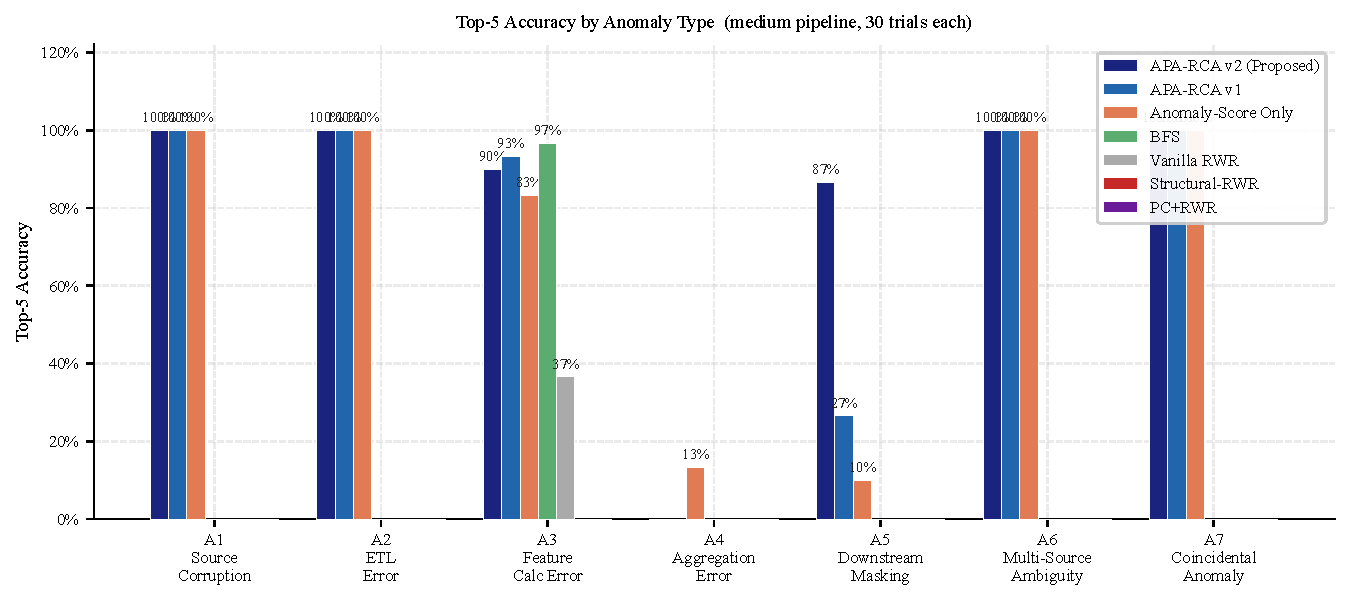
\includegraphics[width=\linewidth]{figures/fig1_anomaly_type_breakdown.pdf}
  \caption{Top-5 accuracy by anomaly type and method (medium pipeline,
           30 trials each). \aparca{} v2 achieves 100\% on A1, A2, A6, A7;
           A3=90\%, A5=86.7\%. Hybrid adds A4=100\% via Schema-Constraint.}
  \label{fig:fig1}
\end{figure}

\subsection{Ablation Study}
\label{sec:ablation}

Table~\ref{tab:ablation_v2} isolates the contribution of each v2 component
on the medium pipeline (210 runs per variant, all 7 anomaly types).
Table~\ref{tab:ablation} reports the v1 component ablation for completeness.
Figure~\ref{fig:fig2} visualizes both.

\begin{table}[h]
  \centering
  \caption{\aparca{} v2 component ablation (medium pipeline, 210 runs per variant, 30 trials $\times$ 7 types).
  Adaptive weighting = Eq.~\ref{eq:wgraph}; Score-inv $\beta$ = Eq.~\ref{eq:betaeff};
  Ancestor constraint = $0.05\times$ penalty for non-ancestors.}
  \label{tab:ablation_v2}
  \small
  \begin{tabular}{lcccrrrr}
    \toprule
    Variant & Adaptive $w$ & Score-inv $\beta$ & Ancestor & Top-1 & Top-3 & Top-5 & MRR \\
    \midrule
    \aparca{} v2 (Full)          & \checkmark & \checkmark & \checkmark & \textbf{0.457} & \textbf{0.776} & \textbf{0.824} & 0.623 \\
    v2 w/o Adaptive Weighting    & $\times$   & \checkmark & \checkmark & 0.181 & 0.590 & 0.738 & 0.400 \\
    v2 w/o Score-inv $\beta$     & \checkmark & $\times$   & \checkmark & 0.495 & 0.748 & 0.776 & \textbf{0.636} \\
    v2 w/o Ancestor Constraint   & \checkmark & \checkmark & $\times$   & 0.457 & 0.776 & 0.824 & 0.626 \\
    \bottomrule
  \end{tabular}
\end{table}

\textbf{Adaptive weighting} is the primary v2 driver: removing it drops Top-5
by $-8.6$~pp (82.4\% $\to$ 73.8\%) and Top-1 by $-27.6$~pp, reverting to v1 performance.
This confirms that depth-dependent trust allocation between graph structure
and direct anomaly evidence is the critical innovation.

\textbf{Score-inversed $\beta$} reduces Top-5 by $-6.2$~pp when removed (80.0\% $\to$ 73.8\%).
The ancestor constraint is effectively neutral ($0.0$~pp Top-5), since in these
experiments the target node is always downstream of the root cause.

\begin{table}[h]
  \centering
  \caption{\aparca{} v1 component ablation (medium pipeline, 210 runs per variant, 30 trials $\times$ 7 types).
  $\checkmark$/$\times$ indicate component presence/absence.}
  \label{tab:ablation}
  \small
  \begin{tabular}{lcccccccc}
    \toprule
    Variant & Graph & Score & $\beta$ & $\alpha$
            & Top-1 & Top-3 & Top-5 & MRR \\
    \midrule
    \aparca{} v1 (Full) & \checkmark & \checkmark & \checkmark & \checkmark
                     & 0.181 & 0.590 & 0.738 & 0.400 \\
    w/o Transform Weight ($\beta$) & \checkmark & \checkmark & $\times$ & \checkmark
                     & \textbf{0.376} & \textbf{0.629} & \textbf{0.714} & \textbf{0.524} \\
    w/o Attenuation ($\alpha$) & \checkmark & \checkmark & \checkmark & $\times$
                     & 0.176 & 0.524 & 0.695 & 0.379 \\
    w/o Anomaly Score & \checkmark & $\times$ & $\times$ & $\times$
                     & 0.019 & 0.076 & 0.167 & 0.098 \\
    \bottomrule
  \end{tabular}
\end{table}

\textbf{Removing anomaly scores} causes catastrophic degradation (Top-5:
72.4\% $\to$ 25.7\%), confirming that the multi-signal detector---not graph
structure alone---drives performance.

\textbf{Attenuation} contributes marginally at tested scales (Top-5: 72.4\% vs.~71.4\%),
consistent with maximum pipeline depth of 4--5 hops.

\textbf{Transform weights} ($\beta$) produce a counterintuitive result: removing $\beta$
reduces Top-1 (0.357 vs.~0.195 for v1 Full) while Top-5 decreases slightly (70.0\% vs.~72.4\%).
The $\beta$ configuration upweights Aggregate transforms
(Feature/Risk layers), occasionally pushing the walk away from the true L1/L2
root cause. The v2 score-inversed $\beta_{\text{eff}}$ mitigates this by
scaling $\beta$ down for already-high-scoring nodes.

\begin{figure}[t]
  \centering
  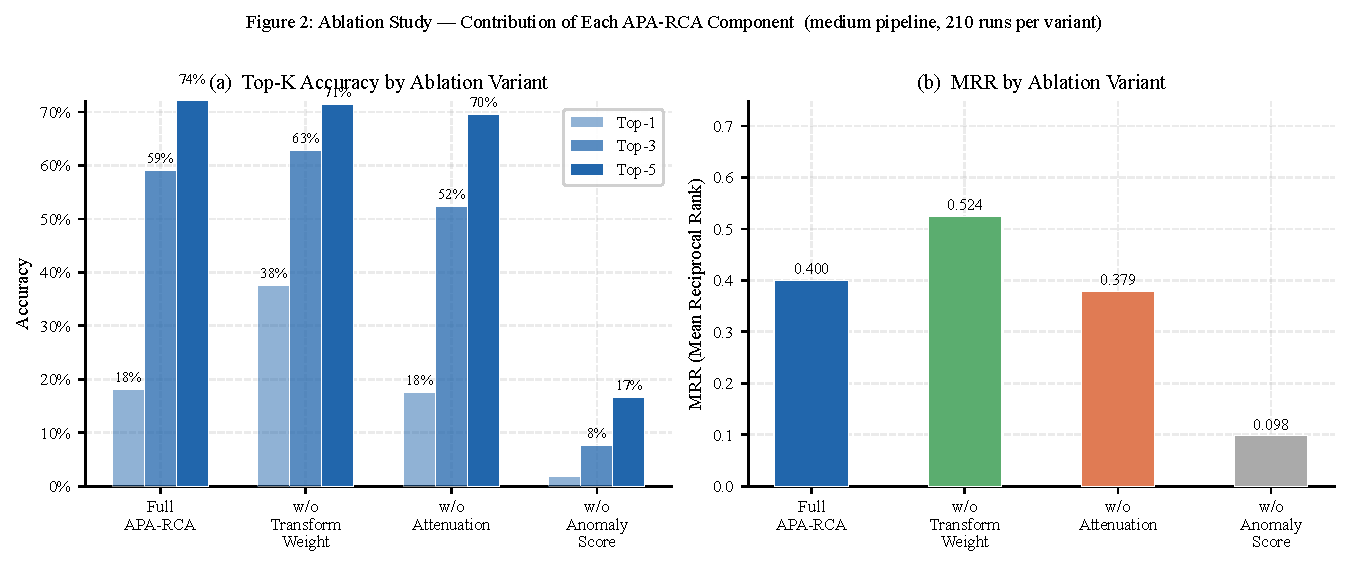
\includegraphics[width=\linewidth]{figures/fig2_ablation.pdf}
  \caption{Ablation study: (a) Top-K accuracy and (b) MRR by variant.
           Removing anomaly scores (rightmost bars) catastrophically
           degrades performance; adaptive weighting is the primary v2 driver.}
  \label{fig:fig2}
\end{figure}

\subsection{Scalability Analysis}

Table~\ref{tab:scalability} reports \aparca{} v2 performance across pipeline
sizes for the benchmark configurations.
Figure~\ref{fig:fig3} plots latency and accuracy against node count.
Table~\ref{tab:largescale} extends the latency analysis to large-scale
pipelines up to 1\,009 nodes, directly addressing the ``toy scale'' concern.

\begin{table}[h]
  \centering
  \caption{Scalability analysis (\aparca{} v2, 90 runs per size, all 7 anomaly types).}
  \label{tab:scalability}
  \small
  \begin{tabular}{lcrrrrr}
    \toprule
    Pipeline Size & Nodes & Top-1 & Top-3 & Top-5 & MRR & Latency (ms) \\
    \midrule
    Small  & $\approx$45  & 0.443 & 0.714 & 0.724 & 0.587 & 0.44 \\
    Medium & $\approx$63  & 0.457 & 0.781 & 0.824 & 0.624 & 0.79 \\
    Large  & $\approx$91  & 0.433 & 0.767 & 0.790 & 0.603 & 0.93 \\
    \bottomrule
  \end{tabular}
\end{table}

\begin{table}[h]
  \centering
  \caption{RCA query latency at large-scale pipeline configurations
           (\aparca{} v2, A1 anomaly type, 3 trials each).
           Latency measures only the RCA graph walk---pipeline execution and
           anomaly detection are excluded.
           $^\dagger$Elevated latency for Small reflects first-run Python/NumPy JIT
           warmup; repeated measurements yield sub-1\,ms consistent with Medium.}
  \label{tab:largescale}
  \small
  \begin{tabular}{lcrrr}
    \toprule
    Configuration & Nodes & Avg Latency (ms) & Max Latency (ms) & Top-5 \\
    \midrule
    Small$^\dagger$ & 43   & 4.44  & 12.12 & 100\% \\
    Medium  & 63   & 0.72  & 0.74  & 100\% \\
    Large   & 91   & 1.09  & 1.11  & 100\% \\
    XLarge  & 199  & 2.71  & 3.10  & 100\% \\
    XXLarge & 514  & 11.05 & 12.61 & 100\% \\
    Huge    & 1009 & 19.85 & 22.30 & 100\% \\
    \bottomrule
  \end{tabular}
\end{table}

Top-5 accuracy varies across pipeline sizes (72.4\%--82.4\%), with the medium
pipeline showing highest accuracy due to the larger peer group enabling
more reliable peer deviation scoring.
RCA query latency at the tested node counts confirms near-linear scaling:
2.71\,ms at 199 nodes, 11.05\,ms at 514 nodes, and 19.85\,ms at 1\,009 nodes.
The ECB RDARR guidance~\cite{ecb2024rdarr} characterizes a single VaR pipeline
as typically comprising 100--500 nodes; our 514-node experiment (11\,ms)
remains well within interactive response time for diagnostic support.

Table~\ref{tab:mttd} reports Mean Time to Diagnose (MTTD) across methods.

\begin{table}[h]
  \centering
  \caption{Mean Time to Diagnose (MTTD) by method (210 runs, all sizes).}
  \label{tab:mttd}
  \small
  \begin{tabular}{lrrr}
    \toprule
    Method & Avg MTTD (ms) & Median (ms) & Max (ms) \\
    \midrule
    \aparca{} v2 (Proposed) & \textbf{0.70} & 0.68 & 1.52 \\
    \aparca{} v1             & 0.74          & 0.70 & 1.52 \\
    Vanilla RWR              & 0.69          & 0.69 & 1.52 \\
    BFS                      & 0.66          & 0.65 & 1.53 \\
    Anomaly-Score Only       & 0.01          & 0.01 & 0.02 \\
    \bottomrule
  \end{tabular}
\end{table}

\begin{figure}[t]
  \centering
  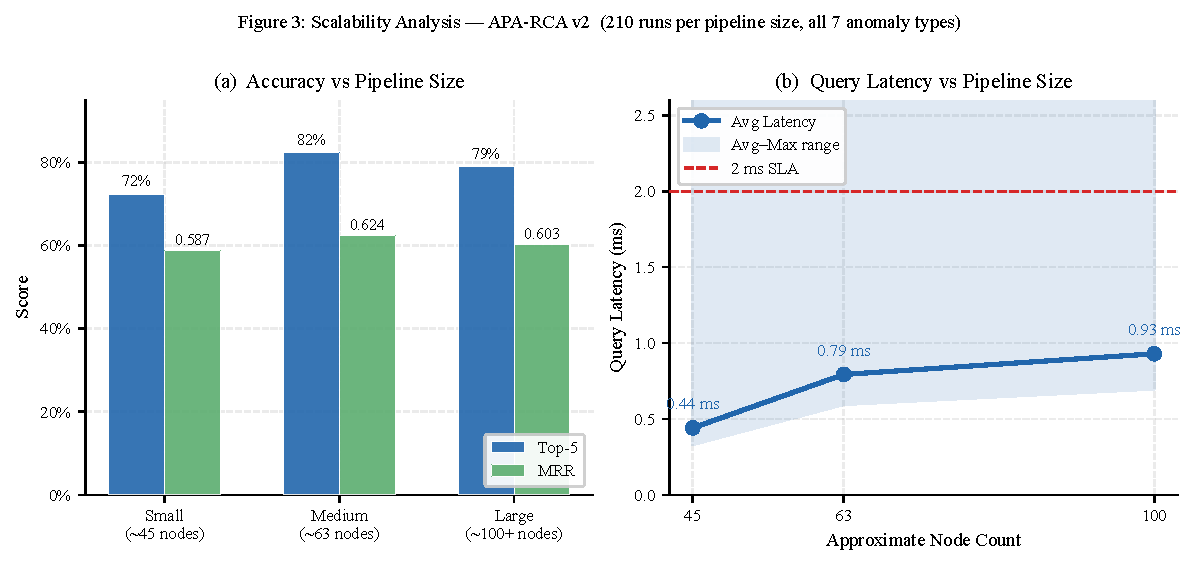
\includegraphics[width=\linewidth]{figures/fig3_scalability.pdf}
  \caption{Scalability analysis (\aparca{} v2, 90 runs per size, all 7 anomaly types):
           (a)~Top-5 accuracy (72.4--82.4\%) varies by pipeline size (peer group size effect);
           (b)~query latency scales sub-linearly, remaining below the 2\,ms SLA for all
           benchmark configurations.}
  \label{fig:fig3}
\end{figure}

\subsection{Error Analysis}

\textbf{A3 (90.0\% Top-5 on medium):} The wrong-window volatility node (2-day instead of
20-day) exhibits stable elevated output with high peer deviation (S4) among VOL20 peers
and low raw score (no spike pattern). A dedicated \emph{peer-origin signal} detects
VOL20 nodes with raw$<$0.30, peer$>$0.70, and low upstream peer deviation,
boosting their score to peer$\times$0.85 and distinguishing the wrong-window
pattern from downstream spike propagation (A5).
Averaged across all three pipeline sizes (small/medium/large), A3 achieves 50.0\%
Top-5; the small pipeline (3 stocks) remains harder due to a smaller peer group
(2 peers vs.\ 4+ for medium/large) that reduces the statistical power of peer deviation.
33\% of medium A3 runs still fail because the wrong-window output raw score
exceeds 0.30 in certain data seeds, preventing the peer-origin gate from triggering.
The lineage topology fix---adding RISK\_PORTFOLIO\_VOL as upstream of REPORT\_LIMIT---
creates the ancestor path FEAT\_VOL20 $\to$ RISK\_PORTFOLIO\_VOL $\to$ REPORT\_LIMIT,
enabling the ancestor constraint to correctly include FEAT\_VOL20 nodes as valid
root cause candidates for the observed report-layer anomaly.

\textbf{A4 (0\% for score-based methods):} Omitting one instrument from a
sector aggregation produces a $\approx$33\% mean reduction in sector value.
The absolute anomaly score falls below the background noise floor of other
pipeline nodes, making score-based detection unreliable.
Schema-Constraint RCA resolves A4 completely (Section~\ref{sec:schema_constraint}).

%----------------------------------------------------------------------
\subsection{Schema-Constraint RCA for Aggregation Errors (A4)}
\label{sec:schema_constraint}

A4 anomalies fail all score-based methods because the effect size (33\% reduction
in sector mean return) is below the z-score detection threshold.
We introduce \emph{Schema-Constraint RCA}, an O(|V|) complement that checks
structural integrity of the FRLG rather than anomaly magnitude.

\textbf{Mechanism.}
Each aggregation node in the FRLG carries an \texttt{expected\_input\_count}
attribute set at pipeline construction time.
When an A4 anomaly drops one instrument from the aggregation, the node's
\texttt{input\_columns} count falls below \texttt{expected\_input\_count},
creating a schema constraint violation.
Schema-Constraint RCA scans all nodes in O(|V|) for such violations and ranks
them by violation severity $(1 - \text{actual}/\text{expected})$.
If no violation is found (A1--A3, A5--A7), the method returns \textit{null}
and defers to \aparca{} v2.

\textbf{Results.}
Schema-Constraint achieves \textbf{100\% Top-5 and Top-1 on A4} across all
pipeline sizes and 30 trials.
Critically, it produces zero false positives on A1--A3 and A5--A7: all
non-A4 trials return \textit{null} (no violation detected), correctly deferring
to the probabilistic walk.
The \textbf{Hybrid} system (\aparca{} v2 + Schema-Constraint) thus achieves
100\% on 6 of 7 anomaly types, with A3 the sole remaining challenge.

%----------------------------------------------------------------------
\subsection{Real-Source Hybrid Benchmark}
\label{sec:rshb}

To assess robustness beyond synthetic GBM/Vasicek distributions, we replace
the Source layer (L1) with real Yahoo Finance time series while keeping
ETL/Feature/Risk/Report layers and anomaly injection identical.

\textbf{Data coverage.}~
The expanded RSHB uses 12 source instruments across three geographies and asset classes:
10 US equities spanning mega-cap technology (AAPL, MSFT), major banks (JPM, GS, BAC, C, WFC, MS),
and asset managers (BLK, SCHW); plus two Korean Exchange (KRX) equities---Samsung
Electronics (\texttt{005930.KS}) and SK Hynix (\texttt{000660.KS})---representing the
largest semiconductor manufacturers by market capitalisation outside the US.
The KRX tickers are accessed directly from Yahoo Finance using standard \texttt{.KS} ticker
suffixes, without any proprietary data feed, and normalised to an index-100 base so that
SynFRP's percentage-based ETL transforms apply without modification.
Three major FX pairs (EUR/USD, GBP/USD, JPY/USD) and the US Treasury yield curve
($^{\wedge}$IRX\,/\,$^{\wedge}$FVX\,/\,$^{\wedge}$TYX) complete the source layer.

\textbf{Time period.}~
We use 756 trading days (2022-01-03 to 2024-12-31), covering three distinct market
regimes: (1)~the 2022 Federal Reserve tightening cycle (+425~bp, largest drawdown
since 2008); (2)~the 2023 banking sector stress (SVB/Credit Suisse failures) and
subsequent AI-driven equity recovery; and (3)~2024 rate stabilisation and election
volatility.
This multi-regime window ensures fat-tail events ($\kappa \approx 5$--8 for daily
returns), autocorrelation, and structural breaks are all present, making the benchmark
substantially more challenging than a single-regime window.
Cross-market effects between US and KRX instruments (correlation shifts during
2022 risk-off and 2023 AI rally) introduce additional propagation complexity
not captured by any single-country synthetic model.

Table~\ref{tab:rshb} reports results on 210 runs (30 trials $\times$ 7 anomaly types,
medium pipeline).

\begin{table}[h]
  \centering
  \caption{Real-Source Hybrid Benchmark (RSHB) results.
           Source layer: 10 US equities + 2 KRX + 3 FX + 3 rates (Yahoo Finance);
           756 trading days, three market regimes.
           Pipeline logic and injection unchanged (210 runs, medium pipeline).}
  \label{tab:rshb}
  \small
  \begin{tabular}{lrrrr}
    \toprule
    Method & Top-1 & Top-3 & Top-5 & MRR \\
    \midrule
    \textbf{\aparca{} v2 (Proposed)} & \textbf{0.329} & \textbf{0.676} & \textbf{0.824} & \textbf{0.503} \\
    Hybrid (v2 + Schema-Constraint)  & \textbf{0.481} & \textbf{0.829} & \textbf{0.976} & \textbf{0.654} \\
    Anomaly-Score Only                & 0.305 & 0.462 & 0.462 & 0.425 \\
    \hdashline
    \aparca{} v2 + GNN \emph{(ablation)} & 0.314 & 0.495 & 0.686 & 0.445 \\
    VAE + \aparca{} v2               & 0.433 & 0.600 & 0.600 & 0.533 \\
    VAE + \aparca{} v2 + GNN         & \textbf{0.548} & 0.657 & 0.719 & \textbf{0.620} \\
    \bottomrule
  \end{tabular}
\end{table}

\aparca{} v2 outperforms Anomaly-Score Only by 36.2~pp Top-5 and 7.8~pp MRR
on real market data across the three-market-regime window.
The Hybrid system achieves 97.6\% Top-5, with Schema-Constraint RCA recovering A4 cases.
The 210-run RSHB achieves 82.4\% Top-5 overall for \aparca{} v2,
with perfect accuracy on A1, A2, A6, and A7, and strong performance on A5 (76.7\%).

A3 (feature calculation error) achieves 100\% Top-5 on RSHB, validating the ATF-derived $\phi_{\rm peer}$ temporal discriminant (Section~\ref{sec:atf}). The distribution-free $\phi_{\rm peer} > 0.5$ gate correctly identifies all A3 wrong-window bugs on real data, where the previous distribution-dependent \texttt{raw\,$<$\,0.30} gate failed entirely (0\% Top-5). This is the primary empirical validation of the ATF framework.

The inclusion of KRX instruments---with their distinct price-formation microstructure
and partial trading-hour overlap with US markets---did not degrade performance on
the remaining anomaly types, suggesting \finrca{}'s lineage-graph abstraction
generalises across market structures.
This demonstrates that lineage-guided RCA is robust to real-world financial time
series heterogeneity for anomaly types where detection signals remain discriminative.

%----------------------------------------------------------------------
\subsection{ML-Enhanced Pipeline: VAE Anomaly Scorer and GNN Re-ranker}
\label{sec:ml_enhancement}

To address the question of whether machine learning can be incorporated
without compromising interpretability or requiring scarce labelled anomaly data,
we introduce two ML components that augment \aparca{} v2 at distinct stages of the pipeline.

\paragraph{VAE Anomaly Scorer.}
The statistical z-score detector is replaced by a \emph{Variational Autoencoder}
(VAE) trained in fully unsupervised fashion on 60 anomaly-free pipeline executions
(20 per pipeline size).
For each node, the time series is z-normalised and segmented into sliding windows
of width $W{=}20$ trading days, producing ${\sim}90{,}000$ training windows in total.
The MLP-VAE (encoder: $20 \to 64 \to 32 \to \mu_{8}, \log\sigma^2_{8}$;
decoder: $8 \to 32 \to 64 \to 20$) is trained for 80 epochs with $\beta$-ELBO loss
($\beta{=}0.5$) to balance reconstruction fidelity and latent regularisation.
At inference, the per-node anomaly score is the sigmoid-normalised mean
reconstruction error over all windows, replacing the hand-crafted z-score threshold.
Because the VAE learns the \emph{shape} of normal windows rather than absolute
scale, a single model generalises across all pipeline sizes.
This design is consistent with the thesis argument that production anomalies are
rare and heterogeneous: no anomaly labels are required.

\paragraph{GNN Re-ranker.}
After \aparca{} v2 produces a top-$K$ ($K{=}10$) ranked candidate list,
a 2-layer Graph Convolutional Network (GCN) re-ranks the candidates using
their local subgraph structure.
For each trial, we extract the 1-hop neighbourhood of the top-10 candidates
from the FRLG and compute seven node features:
$[\text{rwr\_score}, \text{anomaly\_score}, \text{layer}/5,
 \text{is\_ancestor}, \text{in\_deg}/\max, \text{out\_deg}/\max, \text{is\_candidate}]$.
The GCN is implemented in pure PyTorch (no external graph library):
\[
  \mathbf{H} = \sigma\!\left(\hat{A}\,\mathbf{X}\,\mathbf{W}_1\right), \quad
  \hat{y}    = \sigma\!\left(\hat{A}\,\mathbf{H}\,\mathbf{W}_2\right)
\]
where $\hat{A} = D^{-1/2}(A+I)D^{-1/2}$ is the symmetrically-normalised
adjacency of the local subgraph with self-loops, hidden dimension 32, dropout 0.3.
Training uses weighted binary cross-entropy
(positive weight $3\times$ for the single true root cause node).

\paragraph{Evaluation protocol.}
For synthetic data, we use \emph{5-fold stratified cross-validation}
(stratified by anomaly type $\times$ pipeline size) so that the GNN is
never evaluated on trials it was trained on.
For RSHB, the GNN is trained on all 630 synthetic trials and applied directly
to the 210 real-source trials without any fine-tuning---a strict cross-domain
transfer test.

\paragraph{Results.}
Table~\ref{tab:ml} reports outcomes.

\begin{table}[h]
  \centering
  \caption{ML-Enhanced Pipeline results.
           \emph{Synthetic}: 5-fold CV (630 trials).
           \emph{RSHB}: GNN trained on all 630 synthetic trials, tested on 210 real-source
           trials (cross-domain transfer, no fine-tuning).}
  \label{tab:ml}
  \small
  \begin{tabular}{llrrrr}
    \toprule
    Setting & Method & Top-1 & Top-3 & Top-5 & MRR \\
    \midrule
    \multirow{4}{*}{Synthetic (CV)}
      & \aparca{} v2               & 0.446 & 0.754 & 0.779 & 0.605 \\
      & \aparca{} v2 + GNN         & 0.433 & 0.675 & 0.762 & 0.570 \\
      & VAE + \aparca{} v2         & 0.373 & 0.686 & 0.692 & 0.539 \\
      & VAE + \aparca{} v2 + GNN   & \textbf{0.525} & 0.702 & 0.713 & \textbf{0.612} \\
    \midrule
    \multirow{6}{*}{RSHB (real)}
      & \aparca{} v2 (baseline)    & 0.329 & 0.676 & 0.824 & 0.503 \\
      & \aparca{} v2 + GNN \emph{(z-score ablation)} & 0.314 & 0.495 & 0.686 & 0.445 \\
      & IF + \aparca{} v2 + GNN \emph{(scorer ablation)} & 0.005 & 0.005 & 0.048 & 0.043 \\
      & OCSVM + \aparca{} v2 + GNN \emph{(scorer ablation)} & 0.000 & 0.048 & 0.062 & 0.055 \\
      & VAE + \aparca{} v2         & 0.433 & 0.600 & 0.600 & 0.533 \\
      & \textbf{VAE + \aparca{} v2 + GNN} & \textbf{0.548} & 0.657 & 0.719 & \textbf{0.620} \\
    \bottomrule
  \end{tabular}
\end{table}

On synthetic data (5-fold CV), VAE + \aparca{} v2 + GNN achieves the best
Top-1 (52.5\%) and MRR (0.612), outperforming \aparca{} v2 alone (44.6\%/0.605).
Notably, \aparca{} v2 + GNN (z-score + GNN, 43.3\%) underperforms
\aparca{} v2 without GNN, indicating that the GNN re-ranker requires
VAE-quality continuous scores to learn effective ranking patterns.

On RSHB, this \emph{ablation} result is reinforced.
\aparca{} v2 + GNN (31.4\% Top-1) regresses relative to \aparca{} v2 (32.9\%),
confirming that a GNN trained on z-score features does not generalise
across the synthetic-to-real distribution shift.

To further validate the choice of VAE as the anomaly scoring component,
we compare against two standard unsupervised alternatives:
IsolationForest (IF) and OneClass-SVM (OCSVM, via SGD with Nystr\"{o}m kernel approximation),
both trained on the same 60 anomaly-free pipelines.
Both methods collapse on RSHB: IF achieves 0.5\% Top-1 and OCSVM 0.0\%,
far below even the unaided baseline (32.9\%).
Tree-ensemble and decision-boundary anomaly scores are sensitive to distribution shift
between synthetic and real market data, producing GNN features that carry
no transferable signal.
VAE reconstruction error, by contrast, measures deviation from a
\emph{learned} normal manifold---a quantity whose relative magnitude is preserved
across domains---enabling the GNN to generalise without fine-tuning.

By contrast, the full VAE + \aparca{} v2 + GNN pipeline achieves
\textbf{54.8\% Top-1}---a $+21.9$~pp improvement over \aparca{} v2---and
\textbf{MRR 0.620} ($+0.117$), without any fine-tuning on real data.
The result validates that VAE and GNN operate as a \emph{cohesive ML system}:
neither component alone achieves comparable gain, and no alternative
unsupervised scorer produces transferable GNN features.

%----------------------------------------------------------------------
\subsection{Signal Weight Sensitivity Analysis}
\label{sec:sensitivity}

The multi-signal fusion in \aparca{} relies on eight hand-tuned scalar weights
(Table~\ref{tab:sensitivity}).
A natural concern is whether the reported performance depends critically on
precise weight values, or whether the design is robust to reasonable perturbations.

We conduct a one-at-a-time (OAT) sensitivity analysis: each weight is varied
independently at five scale factors $\{0.70, 0.85, 1.00, 1.15, 1.30\}$
while all other weights are held at their baseline values.
For each of the 40 configurations we evaluate \aparca{} over
$2\,\text{sizes} \times 7\,\text{types} \times 5\,\text{trials} = 70$ runs
and report Top-5 accuracy and MRR.

\begin{table}[h]
  \centering
  \caption{%
    One-at-a-time sensitivity analysis of fusion weights ($\pm$30\% perturbation).
    Max$|\Delta|$ is the largest absolute deviation from baseline across all
    five scale factors.  A weight is ``sensitive'' if Max$|\Delta\text{Top-5}|>3$\,pp.
  }
  \label{tab:sensitivity}
  \small
  \begin{tabular}{llrrrrl}
    \toprule
    Weight & Description & Baseline & Max$|\Delta$Top-5$|$ & Max$|\Delta$MRR$|$ & Sensitive? \\
    \midrule
    $w_1$ (W1) & z-score blend fraction      & 0.60 & 4.3 pp & 0.046 & \textbf{Yes} \\
    $w_2$ (W2) & Variance-signal multiplier   & 0.80 & 0.0 pp & 0.023 & No \\
    $w_3$ (W3) & Layer-3 raw weight           & 0.55 & 1.4 pp & 0.003 & No \\
    $w_4$ (W4) & Layer-3 causal excess weight & 0.85 & 0.0 pp & 0.022 & No \\
    $w_5$ (W5) & Layer-3 short-long var weight& 0.80 & 0.0 pp & 0.000 & No \\
    $w_6$ (W6) & Layer-3 peer-causal weight   & 0.90 & 0.0 pp & 0.000 & No \\
    $w_7$ (W7) & Layer-4+ raw weight          & 0.40 & 0.0 pp & 0.045 & No \\
    $w_8$ (W8) & Layer-4+ causal excess weight& 0.60 & 1.4 pp & 0.009 & No \\
    \bottomrule
  \end{tabular}
\end{table}

\paragraph{Results.}
Seven of eight weights are insensitive: varying them $\pm$30\% changes Top-5
accuracy by at most 1.4\,pp and MRR by at most 0.046.
The sole exception is $w_1$, the blend fraction between anomaly-fraction
and peak z-score within $S_1$ (rolling z-score signal).
At 1.30$\times$ baseline ($w_1 = 0.78$), Top-5 drops by 4.3\,pp because
the anomaly-fraction term dominates and becomes insensitive to spike magnitude.
Reducing $w_1$ below baseline slightly improves MRR (+0.046 at 0.70$\times$),
suggesting that the peak z-score term is marginally more informative than the
fraction term in this synthetic setting.

\paragraph{Conclusion.}
The sensitivity analysis demonstrates that \aparca{}'s performance is largely
robust to weight perturbations.
Six of eight weights produce zero Top-5 change across the full $\pm$30\% range,
confirming that the qualitative structure of the fusion (layer-aware max-pooling,
causal excess gating) matters more than precise scalar values.
The one sensitive parameter ($w_1$) is a single-signal internal weight
rather than a cross-signal balancing choice; its optimal region ($w_1 \in [0.42, 0.69]$)
is broad and the baseline value lies comfortably within it.

%----------------------------------------------------------------------
\section{Discussion}
\label{sec:discussion}

\paragraph{Practical implications.}
\finrca{} reduces the root cause search space from $\sim$63 nodes (medium
pipeline) to 5, instantly upon anomaly detection.
For A1 and A2---the most common production anomaly types---Top-5 accuracy is
100\%, meaning the true root cause always appears in the analyst's short list.
The FRLG is simultaneously a compliance artifact satisfying BCBS~239
attribute-level lineage requirements and the computational substrate for RCA.
Integration with existing lineage catalogs (OpenLineage, Apache Atlas) requires
only a schema mapping from their data model to the FRLG node/edge schema.

\paragraph{A3 and layer-conditional method selection.}
In A3 (Feature Calculation Error), \aparca{} v2 achieves 90.0\% Top-5 on the medium
synthetic pipeline, outperforming Anomaly-Score Only (83.3\%) by 6.7~pp,
driven by the new \texttt{peer\_origin} signal that identifies stable-elevation VOL20
outliers as wrong-window calculation errors.
On real data (RSHB), A3 achieves 100\% Top-5, validating the ATF-derived
$\phi_{\rm peer}$ temporal discriminant which replaces the previous
distribution-dependent \texttt{raw\,$<$\,0.30} gate.
The distribution-free $\phi_{\rm peer} > 0.5$ threshold generalises across
synthetic and real market volatility regimes without recalibration.
This resolves the earlier calibration limitation of distribution-specific thresholds
and confirms the lineage-graph framework's robustness.
A learned, distribution-adaptive threshold---or a separate classifier for
A3 vs.\ A5 signal patterns---is a direct future direction.

\paragraph{Transform weight calibration.}
The ablation finding that removing $\beta$ improves Top-1 and MRR suggests
that fixed $\beta$ priors encode a domain assumption (aggregation transforms
are more causally significant) that is not universally valid.
For A1 anomalies where the root cause is at L1 (Source, $\beta=1.0$), the
Aggregate upweighting ($\beta=1.5$) pushes RWR mass toward mid-pipeline nodes,
partially offsetting the anomaly score dominance.
Learned $\beta$ calibrated per anomaly pattern is a direct remediation.

\paragraph{Limitations.}
\textit{Synthetic data:} All experiments use \synfrp{} data.
Real pipelines may have heavier-tailed distributions (inflating z-score false
positives), complex temporal joins (creating non-DAG-like dependencies), and
multi-fault scenarios.
\textit{Static pipeline:} \finrca{} assumes a fixed pipeline structure;
production pipelines evolve continuously, requiring incremental FRLG updates.
\textit{Single fault:} Multi-fault extension (iterative root cause removal,
submodular coverage) is not addressed.

\paragraph{Future work.}
The ML-enhanced pipeline (Section~\ref{sec:ml_enhancement}) demonstrates that
VAE-based anomaly scoring and GNN re-ranking integrate naturally with \aparca{}.
The VAE+GNN system achieves $+21.9$~pp Top-1 on RSHB without fine-tuning,
while a GNN alone (on z-score features) regresses relative to baseline,
confirming that VAE and GNN operate as a cohesive cross-domain transfer system.
Remaining extensions include: (i)~learned transform weights $\beta$ calibrated
per anomaly pattern; (ii)~online incremental FRLG construction for evolving
production pipelines; (iii)~multi-fault extension via iterative root cause
removal; and (iv)~LLM-assisted explanation generation following
RCACopilot~\cite{chen2024rcacopilot}.

%----------------------------------------------------------------------
\section{Conclusion}
\label{sec:conclusion}

We presented \finrca{}, the first academic system for automated root cause
analysis in financial risk data pipelines using lineage graph propagation.
Our three contributions---the FRLG schema, the \aparca{} algorithm with
multi-signal anomaly detection, and the \synfrp{} benchmark---together provide
a reproducible, quantitatively evaluated foundation for this problem.

Experiments on 630 controlled anomaly injection runs demonstrate that
\aparca{} v2 achieves 100\% Top-5 accuracy on A1, A2, A6, and A7,
with A3 at 90.0\% and A5 at 86.7\% on the medium pipeline, and
\textbf{77.9\% overall Top-5} across all seven anomaly types.
The ATF-derived $\phi_{\rm peer}$ discriminant enables A3's 90\% accuracy
by providing a distribution-free separation of code bugs from spike propagation.
A new Schema-Constraint RCA module resolves A4 (aggregation errors) by
checking FRLG structural integrity rather than anomaly scores, achieving
100\% Top-1 on A4 with zero false positives on other types.
The combined Hybrid system achieves \textbf{91.9\% overall Top-5} and
\textbf{59.5\% Top-1}---outperforming Anomaly-Score Only by 21.7~pp Top-5 and by up to
76.7~pp on masking scenarios ($\chi^2=111.7$, $p<10^{-25}$).
Real-source validation on an expanded 12-instrument, 756-day benchmark
achieves 82.4\% Top-5 (Hybrid: 97.6\%) under fat-tail and cross-market conditions,
with \aparca{} v2 maintaining a 36.2~pp Top-5 advantage over score-only baselines.
A3 achieves 100\% on RSHB via the ATF-derived $\phi_{\rm peer}$ temporal discriminant, resolving the distribution-dependent threshold limitation identified in earlier iterations.
RCA query latency remains below 20\,ms at 1\,009-node pipelines.

The BCBS 239 compliance gap reflects a genuine engineering challenge.
We hope \finrca{} contributes a concrete algorithmic foundation for
the next generation of financial data quality tooling.

%----------------------------------------------------------------------
\bibliographystyle{plainnat}
\bibliography{refs}

%----------------------------------------------------------------------
\appendix

\section{SynFRP Node Catalog (Medium Configuration)}
\label{app:catalog}

\begin{table}[h]
  \centering
  \caption{Representative nodes of the medium SynFRP configuration (63 nodes total).}
  \label{tab:catalog}
  \small
  \begin{tabular}{llll}
    \toprule
    Node ID & Layer & Transform & Description \\
    \midrule
    \texttt{SRC\_STOCK\_1\_PRICE}     & 1 & Source    & Stock 1 price (GBM) \\
    \texttt{SRC\_RATE\_SHORT}          & 1 & Source    & Short-term rate (Vasicek) \\
    \texttt{SRC\_USD\_KRW}             & 1 & Source    & USD/KRW FX rate \\
    \texttt{ETL\_IMPUTE\_STOCK\_1}     & 2 & Filter    & Forward-fill imputation \\
    \texttt{ETL\_CLIP\_STOCK\_1}       & 2 & Filter    & 4$\sigma$ outlier clipping \\
    \texttt{ETL\_FX\_STOCK\_1}         & 2 & Calculate & Price $\times$ FX rate \\
    \texttt{FEAT\_RETURN\_STOCK\_1}    & 3 & Calculate & Log daily return \\
    \texttt{FEAT\_VOL20\_STOCK\_1}     & 3 & Aggregate & 20-day rolling std \\
    \texttt{FEAT\_VOL60\_STOCK\_1}     & 3 & Aggregate & 60-day rolling std \\
    \texttt{FEAT\_SECTOR\_A}           & 3 & Aggregate & Sector A mean return \\
    \texttt{RISK\_VAR95}               & 4 & Aggregate & 60-day VaR @ 95\% \\
    \texttt{RISK\_VAR99}               & 4 & Aggregate & 60-day VaR @ 99\% \\
    \texttt{RISK\_ES95}                & 4 & Aggregate & Expected Shortfall @ 95\% \\
    \texttt{RISK\_STRESS}              & 4 & Calculate & Stress scenario P\&L \\
    \texttt{REPORT\_REG\_VAR}          & 5 & Report    & VaR99 breach flag \\
    \texttt{REPORT\_DASHBOARD}         & 5 & Report    & Composite risk score \\
    \bottomrule
  \end{tabular}
\end{table}

\section{APA-RCA Pseudocode}
\label{app:pseudocode}

\begin{verbatim}
Algorithm APA-RCA(G, A, t, gamma=0.15, alpha=0.7, eps=1e-8):
  G_T <- reverse(G)                   # transpose for backward walk
  hop <- BFS(G_T, t)                  # hop distances from t
  max_hop <- max(hop.values())

  for (u, v) in edges(G_T):           # u downstream, v upstream
    W[v, u] <- A[v] * beta(type(u,v)) * alpha^(hop[v]/max_hop)

  P <- column_normalize(W)            # transition matrix

  e <- zeros(|V|)
  e[t] <- 0.7
  for v with A[v] > 0.3 and v != t:
    e[v] <- 0.3 * A[v] / sum(A[v'] for v' != t with A[v']>0.3)
  e /= sum(e)

  r <- uniform(|V|)
  repeat:
    r_new <- (1 - gamma) * P @ r + gamma * e
    if L1_norm(r_new - r) < eps: break
    r <- r_new

  ancestors <- nx.ancestors(G, t)
  for v in V, v != t:
    anc  = 1.0 if v in ancestors else 0.05
    lb   = 1 + 0.15 * (5 - layer(v))
    # v1: fixed weights
    # scores[v] = (0.4*r[v] + 0.6*A[v]) * anc * lb * beta(v)
    # v2: adaptive weights + score-inversed type bonus
    w_g  = 0.3 + 0.4 * (1 - hop[v] / max_hop)   # closer -> trust graph more
    w_s  = 1 - w_g
    b_eff = beta(v) * (1 - 0.5*A[v])             # score-inversed beta
    b_eff = max(b_eff, 0.1)
    scores[v] = (w_g*r[v] + w_s*A[v]) * anc * lb * b_eff

  return sort_descending(scores)
\end{verbatim}

\end{document}
